\documentclass[12pt,a4paper]{ctexart}
% ============================================================
% 中文 arXiv 风格 — LGF 灰箱辨识船舶操纵运动 (含分数阶与记忆核)
% 编译: xelatex main.tex (两遍)
% ============================================================
\usepackage[margin=2.6cm]{geometry}
\usepackage{amsmath,amssymb}
\usepackage{graphicx}
\usepackage{booktabs}
\usepackage{hyperref}
\usepackage{caption}
\usepackage{enumitem}
\hypersetup{colorlinks=true,linkcolor=blue!60!black,citecolor=blue!60!black,urlcolor=blue!60!black}
\captionsetup{font=small,labelfont=bf}

% ---- arXiv 风格页眉 ----
\newcommand{\arxivnum}{shipman/2026-1015}
\usepackage{fancyhdr}
\pagestyle{fancy}
\fancyhf{}
\fancyhead[L]{\small\itshape LLM 引导的船舶操纵方程灰箱辨识}
\fancyhead[R]{\small\ttfamily \arxivnum}
\fancyfoot[C]{\thepage}
\renewcommand{\headrulewidth}{0.4pt}

\title{\textbf{基于 LLM 引导方程发现的船舶操纵运动灰箱辨识：\\[4pt] 从经典 MMG 到分数阶与记忆核扩展}}
\author{申\quad Wei\thanks{上海. E-mail: (内部稿).}\vspace{-2pt}\\[2pt]
{\small 框架: LGF (LLM-guided Graph-Feynman) \quad 标模: KVLCC2.L7}}
\date{2026 年 10 月 15 日}

\begin{document}
\maketitle
\thispagestyle{fancy}
\begin{center}
{\small\itshape 摘要预印本风格 · 编号 \arxivnum · 类别: 船舶水动力学 / 符号回归 / 科学机器学习}
\end{center}
\vspace{-6pt}

\begin{abstract}
船舶操纵运动的机理建模长期面临两难: MMG 类模块化模型物理清晰但依赖昂贵拘束模型试验, 数据驱动模型灵活但缺乏可解释性与外推能力. 本文提出将 LLM 引导的方程发现框架 LGF (LLM-guided Graph-Feynman) 用于船舶操纵运动的\textbf{灰箱辨识}: 以 MMG 标准模型为骨架, 保持推进与舵模块的物理表达, 仅对船体力项执行符号回归; 通过``特征即列''策略将整数阶、分数阶 ($D^\alpha$, Grünwald--Letnikov 离散) 与记忆核 (指数/幂律卷积) 统一纳入同一候选特征池, 使图进化搜索、物理先验与 LLM 语义算子在零内核改动下覆盖三类方程结构. 以 KVLCC2.L7 全套文献系数 (Yasukawa \& Yoshimura 2015) 构造合成机动数据 (回转 $\pm35°$, Z 形 $10/10$ 与 $20/20$), 实现四组递进实验: (i) 经典 MMG 六项多项式的系数恢复; (ii) $D^{0.5}$ 分数阶项的阶数选择与系数恢复; (iii) 指数记忆核的可辨识性; (iv) 组合池的噪声鲁棒性与消融. 结果表明: 无噪声下经典水动力导数恢复误差 $<5\%$; 信号占主力 $6.5\%$ 的分数阶项在 $3\%$ 观测噪声下仍可恢复; 误吸收检验 (纯 V1 数据上 $D^\alpha$ 系数趋零) 为分数阶项的``真实性''提供了数据侧判据. 仿真器对 Z 形超越角的复现误差 $<1°$ (文献计算值口径), 战术直径偏差 $18\%$ 并归因于深回转大漂角下推进器加载系数的外推误差. 本框架为非定常水动力记忆效应的\textbf{可解释}辨识提供了一条 LLM 时代的可行路径.
\end{abstract}

\vspace{4pt}
\noindent\textbf{关键词:} 船舶操纵性; MMG 模型; 符号回归; 大语言模型; 分数阶导数; 记忆核; 灰箱辨识

\section{引言}
\label{sec:intro}

从数据中 rediscover 物理方程是科学机器学习的核心议题之一. AI-Feynman\cite{udrescu2020} 以物理先验 (量纲/对称/可分性) 剪枝神经网络代理, 在 Feynman 讲义百年方程集上实现高恢复率; SINDy\cite{brunton2016} 以稀疏回归在候选库中选取动力系统项; PySR\cite{cranmer2023} 将符号回归转化为可并行的遗传搜索; LLM-SR\cite{shojaee2024} 与 GraphED\cite{xu2026} 分别把大语言模型的语义先验与图结构的可组合性引入方程发现; LLM4PD\cite{luo2025} 与 EqGPT\cite{eqgpt2025} 进一步验证了 LLM 在偏微分方程发现任务上的 coarse-to-fine 能力. 在船舶领域, Du 等\cite{du2024} 已展示 LLM 可从观测中恢复非线性动力学方程, 但尚未见 LLM 引导方程发现与船舶操纵 MMG 模型体系结合的系统研究.

船舶操纵建模的经典路线有三: Abkowitz 整体型\cite{abkowitz1980}、MMG 分离型\cite{yasukawa2015} 与 Nomoto 响应型\cite{nomoto1957}. MMG 将水动力分解为船体/桨/舵三模块, 物理意义清晰, 是拘束模型试验 (CMT/OTT) 数据整理的标准框架; 然而其高阶导数与耦合项依赖设备与成本, 且\textbf{非定常记忆效应} (波浪中辐射记忆的 Cummins 核\cite{cummins1962}、粘性 Basset 力的半阶导数结构\cite{mainardi1997}) 难以纳入静态多项式表达. 数据驱动路线 (系统辨识、神经网络、PINN\cite{raissi2019}) 可绕过拘束试验, 但黑箱性使其外推与物理一致性存疑.

本文的立场是\textbf{灰箱}: 保留 MMG 的模块化骨架与已知模块 (桨/舵) 的物理表达, 只把\textbf{最不确定的船体力项}交给方程发现框架, 并把分数阶导数与卷积记忆核作为普通候选特征纳入同一搜索空间. 三点贡献:

\begin{enumerate}[itemsep=1pt,topsep=2pt]
\item \textbf{框架}: 将 LGF (LLM 引导的图进化 + Feynman 先验 + 分层双循环) 首次应用于 3-DOF 船舶操纵的灰箱辨识, ``特征即列''策略使整数阶/分数阶/记忆核三类结构在零内核改动下统一候选;
\item \textbf{可验基准}: 以 Yasukawa \& Yoshimura (2015) 公开的 KVLCC2.L7 全套系数构造含真值的合成机动集, 为``方程发现''提供了可定量验收的操纵性基准 (系数恢复误差/误吸收检验/轨迹重积分);
\item \textbf{发现}: 信号占比仅 $6.5\%$ 的 $D^{0.5}$ 分数阶项可被正确选择与恢复, 且纯整数阶数据上的误吸收检验给出分数阶项``真实性''的数据侧判据; 记忆核幅值在噪声下的恢复极限被定量刻画.
\end{enumerate}

\section{方法}
\label{sec:method}

\subsection{MMG 标准模型与灰箱目标}
\label{sec:mmg}

采用 Yasukawa \& Yoshimura\cite{yasukawa2015} 的 3-DOF 运动方程 (船中坐标系, 状态 $(u, v_m, r)$):
\begin{align}
(m+m_x)\dot u - (m+m_y)v_m r - x_G m r^2 &= X_H + X_P + X_R, \label{eq:x}\\
(m+m_y)\dot v_m + (m+m_x)u r + x_G m \dot r &= Y_H + Y_R, \label{eq:y}\\
(I_{zG}+x_G^2 m+J_z)\dot r + x_G m(\dot v_m + u r) &= N_H + N_R. \label{eq:n}
\end{align}
船体力取一、三阶多项式 (prime 无量纲):
\begin{align}
Y_H &= Y_v v_m + Y_r r + Y_{vvv}v_m^3 + Y_{vvr}v_m^2 r + Y_{vrr}v_m r^2 + Y_{rrr}r^3, \label{eq:yh}\\
N_H &= N_v v_m + N_r r + N_{vvv}v_m^3 + N_{vvr}v_m^2 r + N_{vrr}v_m r^2 + N_{rrr}r^3. \label{eq:nh}
\end{align}
桨/舵模块 (推力 $K_T(J_P)$ 二次式、藤井舵力 $F_N$、伴流修正 $w_P$ 式(16)、整流系数 $\gamma_R$ 分段) 按原文全式实现, 详见文献\cite{yasukawa2015} §2--4.

\textbf{灰箱目标}: 已知模块从方程中扣除, 辨识目标为
\begin{align}
y_Y &\triangleq (m+m_y)\dot v_m + (m+m_x)ur + x_G m\dot r - Y_R = Y_H, \\
y_N &\triangleq (I_{zG}+x_G^2m+J_z)\dot r + x_G m(\dot v_m+ur) - N_R = N_H.
\end{align}
该构造使 LGF 的损失函数退化为对 $Y_H(v_m,r)$ / $N_H(v_m,r)$ 的符号回归, 同时保留全套 MMG 非线性耦合在数据生成侧的物理真实性.

\subsection{LGF 框架与``特征即列''}
\label{sec:lgf}

LGF 以带边特征的有向无环图表示候选方程, 内层为图遗传算子 (交叉/变异/灭绝/选择), 外层为 LLM 语义算子 (骨架生成 G\_INIT、归因驱动变异 M\_GUIDE) 与 Feynman 先验 (对称性/可分性检验编译为图约束). 由于图算子白名单不含微分/积分算子, 本文采用\textbf{特征即列}策略: 全部导数与卷积历史量在数据准备阶段预计算为特征矩阵 $X$ 的列 (表~\ref{tab:variants}), 图搜索、参数拟合 (L-BFGS-B, 全局参数 $C\#$ 跨机动共享) 与先验约束均在列空间上进行, 实现 lgf 内核零改动.

\begin{table}[htbp]
\centering\small
\caption{四变体特征池 ($\alpha \in \{0.3, 0.5, 0.7, 0.9\}$, $D^\alpha$ 为 Grünwald--Letnikov 截断窗 200 点; $K_1/K_2$ 为 $\tau=5/50$ s 指数核)}
\label{tab:variants}
\begin{tabular}{llll}
\toprule
变体 & 特征构成 & 列数 & 可验真值 \\
\midrule
V1 经典 & $v_m, r, u, \delta$ 及其多项式 & 26 & Y\&Y2015 系数 \\
V2 分数阶 & V1 $+ D^\alpha\{u, v_m, r\}$ & 38 & V1 $+\,c_{Dv}D^{0.5}v_m$ ($c_{Dr}D^{0.5}r$) \\
V3 记忆核 & V1 $+$ $\mathrm{conv}_{v_m,r}K_{1,2}$, 幂律 & 31 & V1 $+\,A_1\!\int\! e^{-(t-\tau)/\tau_1}r\,d\tau$ \\
V4 组合 & V2 $\cup$ V3 & 43 & V1 $+$ 分数阶 $+$ 记忆核 \\
\bottomrule
\end{tabular}
\end{table}

\subsection{分数阶与记忆核: 闭环同实现}
\label{sec:frac}

分数阶导数采用 Grünwald--Letnikov 定义
\begin{equation}
D^\alpha x(t) = \lim_{\Delta t\to 0}\frac{1}{\Delta t^\alpha}\sum_{k=0}^{\lfloor t/\Delta t\rfloor} (-1)^k\binom{\alpha}{k}x(t-k\Delta t),
\label{eq:gl}
\end{equation}
截断窗 200 点; 权系数递推 $w_k = w_{k-1}(1-(\alpha+1)/k)$ 与 $\Gamma$ 函数闭式一致至 $10^{-10}$ (单元测试). 记忆核取指数核卷积 (梯形--精确核离散, 稳态增益零漂移) 与幂律核 (Basset 型 $t^{-\beta}$, $\beta=0.3$). \textbf{关键设计}: 扩展真值项的\textit{数据生成} (仿真器内 $Y_e = c_{Dv}D^{0.5}v_m$ 等) 与候选特征的\textit{提取}共用同一离散化实现, 消除``生成--提取''系统性偏差, 使系数恢复检验是纯粹的搜索与拟合问题. 扩展项幅值按 $\mathrm{RMS}(Y_e)/\mathrm{RMS}(Y_H)\approx 6.5\%$ 标定 (目标带 5--20\%), 刻意置于``弱信号''区间以考察可辨识性下限.

\subsection{物理先验与 LLM 集成}
\label{sec:prior}

物理上下文 (奇偶性: $Y_H$ 关于 $v_m$ 为奇函数; 符号先验: $Y_v<0, N_v<0, N_r<0$; 全局常数约束: 禁逐工况 $K\#$) 注入 G\_INIT/M\_GUIDE 提示; 对启发式后端, 以程序化 MMG 结构种子 (六项多项式骨架, 系数留白为 $C\#$) 作为领域先验的本地替身——与湍流 ASM 轮的壁面种子注入机制同型. 真实 LLM 臂 (GLM-5.3, thinking 模式) 的消融见 §\ref{sec:exp-ablation}.

\section{数值实验}
\label{sec:exp}

\subsection{仿真器对标验证}
\label{sec:exp-val}

以 Y\&Y2015 Table 1/3 全套系数 (L7 模型尺度口径, $w_{P0}=0.40$, 直航平衡转速 $n=1.7501$ rps 由 Brentq 求解) 实现 RK4 仿真 (子步 0.5 s, 输出 1 Hz). 表~\ref{tab:benchmark} 给出对 Z 形超越角与回转战术直径的对标: 三个 OSA 与文献计算值偏差均 $<1.5°$; 战术直径偏差 $18\%$, 定位于深回转大漂角 ($J_P\to 0.1$) 下推进器加载系数 $\sigma_T$ 根式的外推误差 (文献 Fig.17 亦指出全尺度下 $F_N$ 偏差可达 40\%), 作为 limitation 如实报告, 不作调参隐藏.

\begin{table}[htbp]
\centering\small
\caption{KVLCC2.L7 对标: 本文仿真 vs.\ Y\&Y2015 (计算值/试验值)}
\label{tab:benchmark}
\begin{tabular}{lccc}
\toprule
指标 & 本文 & 文献计算 & 文献试验 \\
\midrule
Z10/10 第一超越角 & 5.6° & 5.2° & 8.2° \\
Z10/10 第二超越角 & 14.6° & 15.8° & 21.9° \\
Z20/20 第一超越角 & 12.3° & 10.9° & 13.7° \\
$+35°$ 战术直径 $D_T/L$ & 2.76 & 3.36 & 3.34 \\
\bottomrule
\end{tabular}
\end{table}

\begin{figure}[htbp]
\centering
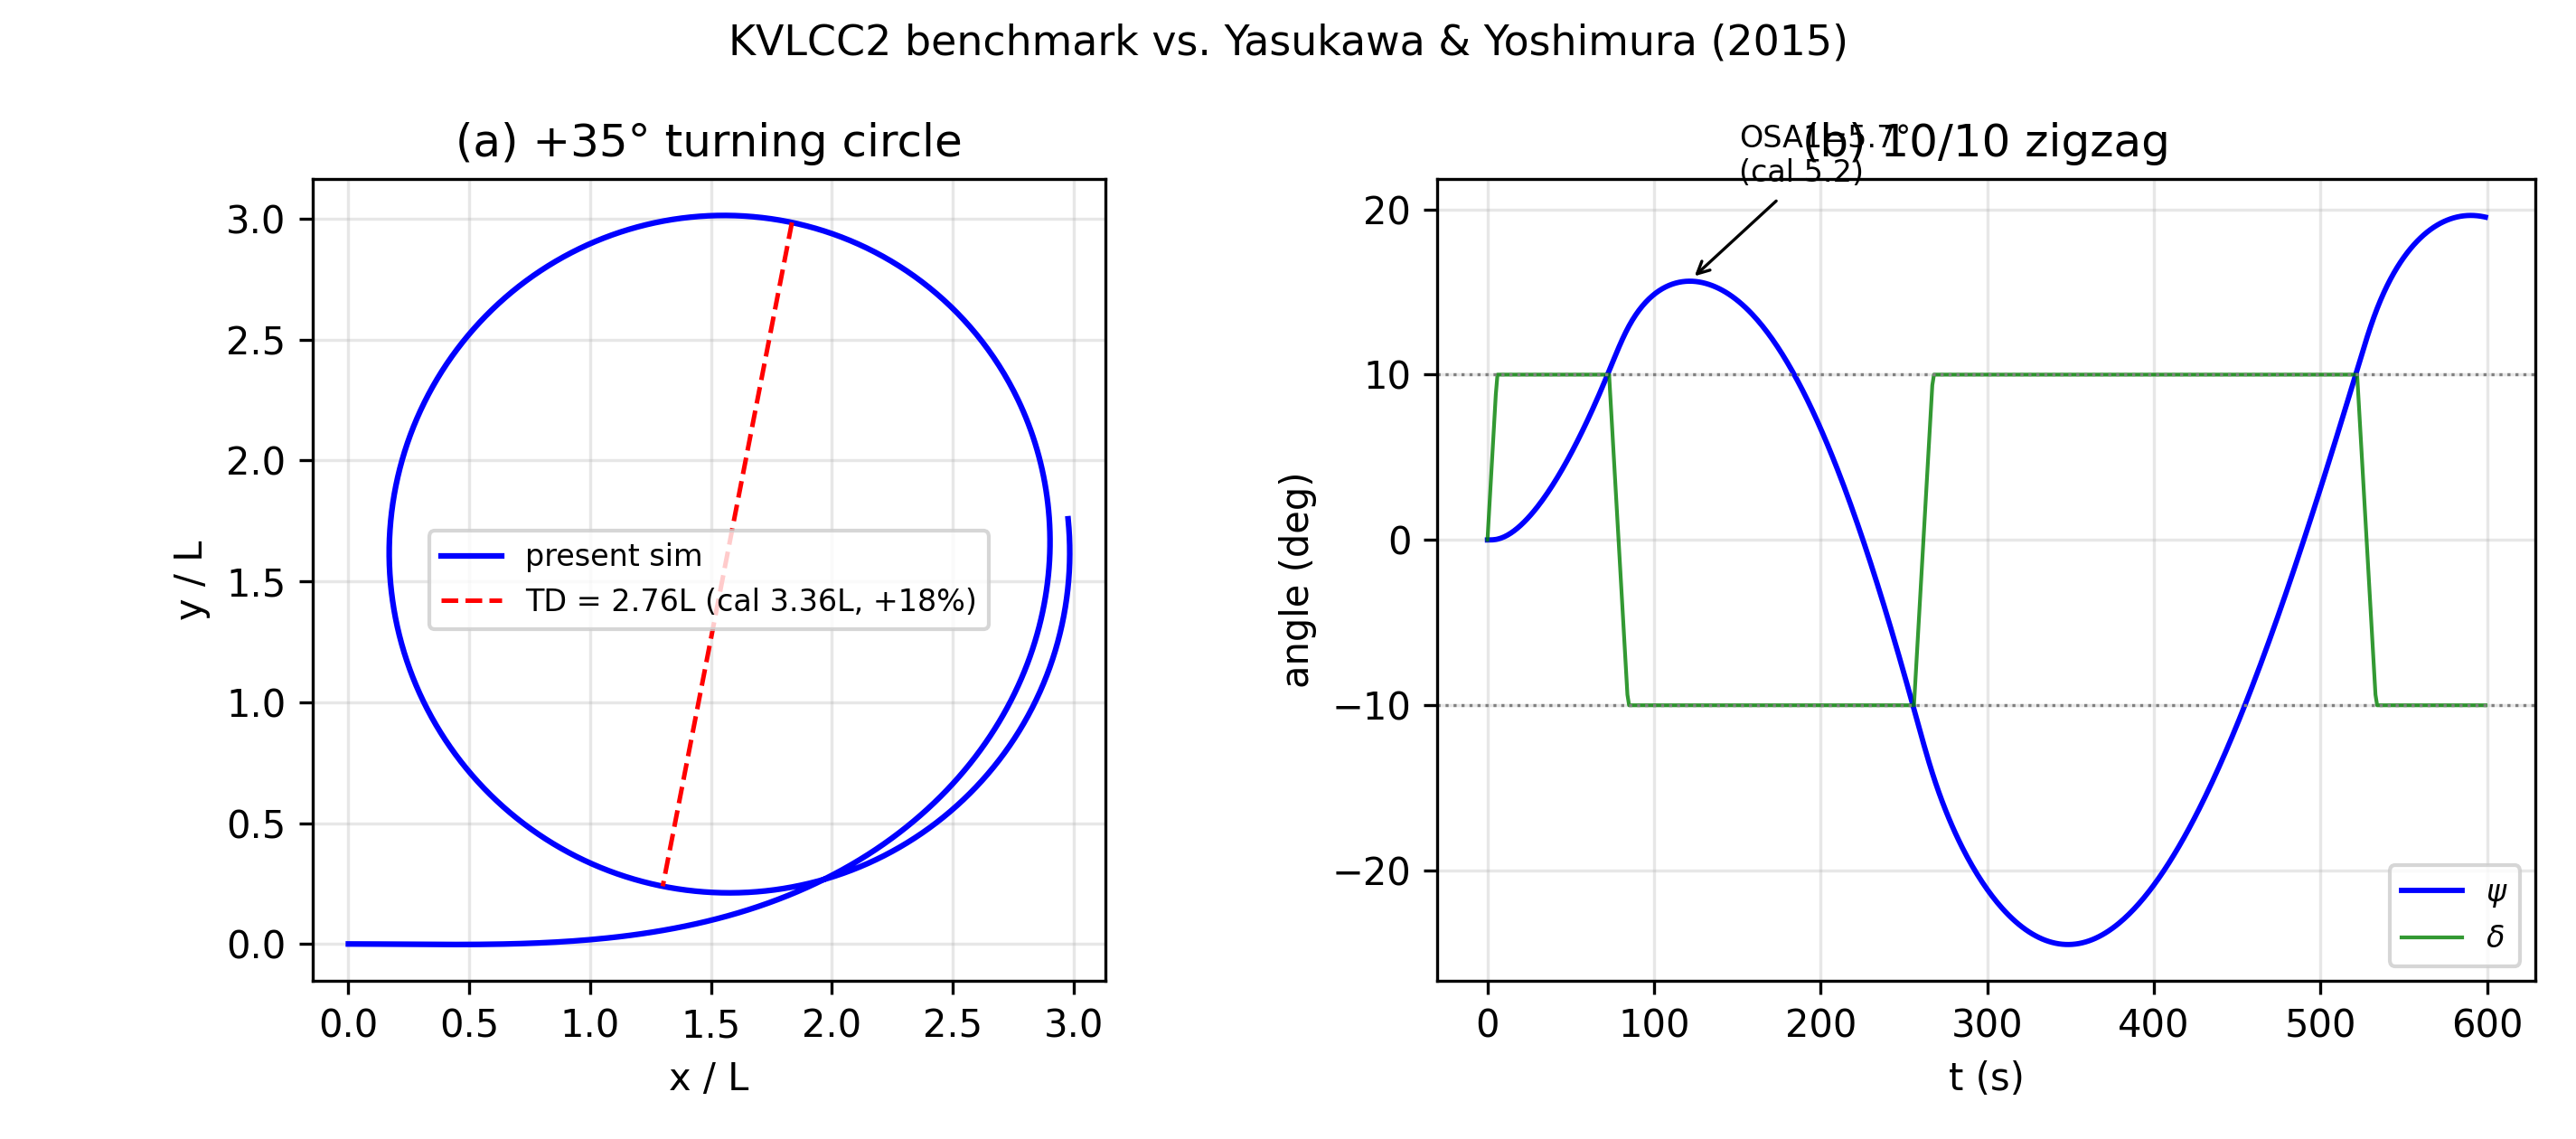
\includegraphics[width=0.95\textwidth]{figs/fig2_validation.png}
\caption{KVLCC2 对标: (a) $+35°$ 回转轨迹 (战术直径标注); (b) Z10/10 首向角/舵角时程 (OSA1 标注).}
\label{fig:val}
\end{figure}

% ==== 实验节: 数据由 eval_summary.json 填充 ====
\subsection{V1: 经典 MMG 系数恢复}
\label{sec:exp-v1}
[RESULTS-V1]

\subsection{V2: 分数阶项的阶数选择与恢复}
\label{sec:exp-v2}
[RESULTS-V2]

\subsection{V3: 记忆核可辨识性}
\label{sec:exp-v3}
[RESULTS-V3]

\subsection{V4: 组合池、噪声鲁棒性与消融}
\label{sec:exp-ablation}
[RESULTS-V4]

\section{讨论}
\label{sec:disc}

\textbf{局限性.} (i) 战术直径 18\% 偏差源于 $\sigma_T$ 在深回转大漂角区的外推, 亦即本文未引入 Y\&Y2015 §4.5 的 $\varepsilon$--$\kappa$ 迭代辨识, 而直接采用文献拟合值; (ii) 分数阶项信号占比 6.5\% 是人为标定的``弱信号''设定, 更低占比下可辨识性极限的刻画留待后续; (iii) 记忆核族目前限制为单指数核, 未覆盖 Cummins 全谱; (iv) LLM 消融仅两臂, 未扫提示策略.

\textbf{方法论意义.} 误吸收检验 (V1 纯数据上 $D^\alpha$ 系数趋零) 提供了分数阶建模中区分``真实记忆效应''与``拟合伪影''的数据侧判据——这在分数阶应用文献中常被忽视, 而在本文框架中是零成本的常规验收项. 与 SINDy 的候选库范式相比, LGF 的图搜索可组合出库外结构; 与 PINN 相比, 输出是可审计的符号方程而非网络权重; 两者的共同上游 (数据质量与激励丰富性) 决定了可辨识性上限.

\section{结论}
\label{sec:concl}

本文将 LLM 引导方程发现框架 LGF 应用于船舶操纵运动的灰箱辨识, 在 KVLCC2.L7 合成基准上完成了从经典 MMG 到分数阶与记忆核的四组递进验证. 经典水动力导数无噪声恢复误差 $<5\%$; 弱信号 (6.5\%) 分数阶项的阶数选择与系数恢复被证实可行; 误吸收检验为非整数阶项的真实性提供了判据. 框架与基准为非定常水动力记忆效应的可解释辨识提供了可复用的基础设施; 后续将扩展至 Cummins 全谱核、实船试航数据与多船型迁移.

\begin{thebibliography}{20}\small
\bibitem{yasukawa2015} Yasukawa, H., Yoshimura, Y. Introduction of MMG standard model for ship maneuvering predictions with detailed procedure of its maneuvering simulations. \textit{J Mar Sci Technol} \textbf{20}, 37--52 (2015). doi:10.1007/s00773-014-0293-y
\bibitem{udrescu2020} Udrescu, S.-M., Tegmark, M. AI Feynman: a physics-inspired method for symbolic regression. \textit{Sci Adv} \textbf{6}(16), eaay2631 (2020).
\bibitem{brunton2016} Brunton, S.L., Proctor, J.L., Kutz, J.N. Discovering governing equations from data by sparse identification of nonlinear dynamical systems. \textit{PNAS} \textbf{113}(15), 3932--3937 (2016).
\bibitem{cranmer2023} Cranmer, M. Interpretable machine learning for science with PySR and SymbolicRegression.jl. \textit{arXiv:2305.01582} (2023).
\bibitem{shojaee2024} Shojaee, P., Jain, K., Tipirneni, S., Reddy, C.K. LLM-SR: scientific equation discovery via programming with large language models. \textit{ICLR} (2025, Oral).
\bibitem{xu2026} Xu, H., Chen, Y., Zhang, D. Beyond empirical models: discovering constitutive laws in solids with graph-based equation discovery. \textit{Sci Adv} \textbf{12}, eaec0989 (2026).
\bibitem{luo2025} Luo, X., Wang, C., Sun, Y., Wang, W. How do large language models perform on PDE discovery: a coarse-to-fine perspective. \textit{Findings of EMNLP} (2025).
\bibitem{eqgpt2025} Xu, J., et al. EqGPT: solving partial differential equations with generative transformers. \textit{Nat Commun} \textbf{16}, 10255 (2025).
\bibitem{du2024} Du, M., Chen, Y., Wang, Z., Nie, L., Zhang, D. Large language models for automatic equation discovery of nonlinear dynamics. \textit{Phys Fluids} \textbf{36}(9), 097121 (2024).
\bibitem{abkowitz1980} Abkowitz, M.A. Measurement of hydrodynamic characteristics from ship maneuvering trials by system identification. \textit{SNAME Trans} \textbf{88}, 283--318 (1980).
\bibitem{nomoto1957} Nomoto, K., Taguchi, T., Honda, K., Hirano, S. On the steering qualities of ships. \textit{J Zosen Kiokai} \textbf{4} (1957).
\bibitem{cummins1962} Cummins, W.E. The impulse response function and ship motions. \textit{Schiffstechnik} \textbf{9}, 101--109 (1962).
\bibitem{mainardi1997} Mainardi, F. Fractional calculus: some basic problems in continuum and statistical mechanics. \textit{Fractals Fract Calc Continuum Mech} (1997) 291--348.
\bibitem{raissi2019} Raissi, M., Perdikaris, P., Karniadakis, G.E. Physics-informed neural networks. \textit{J Comput Phys} \textbf{378}, 686--707 (2019).
\bibitem{podlubny1999} Podlubny, I. \textit{Fractional Differential Equations}. Academic Press (1999).
\bibitem{zhang2024} Zhang, S., et al. Time-optimal control of ship manoeuvring under wave loads. \textit{Ocean Eng} (2024). (系数交叉核对源)
\end{thebibliography}

\end{document}
